\documentclass{article}

\usepackage{graphicx}
\usepackage{mathtools}
\usepackage{amsmath,amsthm,amssymb}
\usepackage{multicol}
\usepackage[skip=3pt]{caption}
\usepackage[top=1in, bottom=1in, left=1in, right=1in]{geometry}
\usepackage{subcaption}
\usepackage{fancyhdr}
\usepackage{tabulary}
\usepackage{times}
\usepackage{datetime}
\usepackage{titling}
%\pagestyle{fancy}
\usepackage[most]{tcolorbox}
\usepackage[T1]{fontenc}
\usepackage[font=small,labelfont=bf,tableposition=top]{caption}
\DeclareCaptionLabelFormat{andtable}{#1~#2  \&  \tablename~\thetable}

\usepackage{algorithm}
\usepackage{algpseudocode}
\algnewcommand\algorithmicforeach{\textbf{for each}}
\algdef{S}[FOR]{ForEach}[1]{\algorithmicforeach\ #1\ \algorithmicdo}
\DeclarePairedDelimiter{\ceil}{\lceil}{\rceil}
\DeclarePairedDelimiter{\floor}{\lfloor}{\rfloor}

\newcommand{\tab}[1][1]{\noindent \hspace{#1cm} }

\usepackage[style=numeric]{biblatex}
\addbibresource{myreferences.bib}

\begin{document}

\noindent \textbf{CSCE 586 - Design and Analysis of Algorithms}

\noindent \textbf{Date:}  \today 

\noindent \textbf{Name:}  Micah Hayden

\noindent \textbf{Assignment:}  Final Exam - Take Home Portion, Version A

\noindent \textbf{Documentation:} 

\hrulefill

\section{Hidden Surface Removal Problem:}
\subsection{Which algorithmic paradigm will you use to solve this problem?}  
I will utilize Divide-and-Conquer to solve this problem.

\subsection{Why did you chose the algorithmic paradigm selected above to solve this problem?}
I believe this paradigm is suited to divide and conquer.  Each line has similar characteristics, following the same equation $y_i = a_i \cdot x + b_i$.  The problem can be divided into small, independent sub-problems using the slope of each line.  The base case occurs when $n \leq 3$:  because no 3 lines intersect at a single point, the resulting "uppermost" lines can be found in constant time.
 
\subsection{Give an algorithm that takes $n$ lines as input, and in $O(n \log{n})$ time returns all of the lines that are visible.  Provide a clear description of the algorithm.}

Let $L$ be a set of lines, $|L|=n$, where $L_i=m_i \cdot x + b_i$. \newline

\noindent Begin by sorting $L$ by ascending slope, such that $L_i$ has slope $m_i$ and $m_i < m_{i+1}$ for all $i$.

\begin{algorithm}
\caption{Hidden-Surface-Removal:  HSR($L$)}
\begin{algorithmic}
\If {$n \leq 2$}
	\State \Return The set of lines $L$, and their intersection $a$.
\ElsIf {$n = 3$}
	\State Let $a =$ the intersection of $L_1$ and $L_3$
	\State Let $b =$ the intersection of $L_1$ and $L_2$
	\If {$x_b < x_a$}
		\State Let $c =$ the intersection of $L_2$ and $L_3$.
		\State \Return $L$ and $\{b, c\}$
	\Else 
		\State \Return $L - \{L_2\}$ and $\{a\}$
	\EndIf
\Else
	\State $R, A = HSR(\{L_1, \dots , L_{\frac{n}{2}}\})$
	\State $R', B = HSR(\{L_{\frac{n}{2}+1}, \dots , L_n\})$
\EndIf
\State Merge $A$ and $B$ into $C$ by increasing $x$ coordinate
\State Find the first element, $c_k$, in $C$ for which the uppermost line of $R' > $ the uppermost line of $R$
\State Let $R_i \in R$ be the uppermost line in $R$ immediately before $c_k$.
\State Let $R'_j \in R'$ be the uppermost line in $R'$ immediately after $c_k$.
\State Let point $p_{int}$ be the intersection of lines $R_i$ and $R'_j$.
\State $L_{final} = \{R_1, R_2, \dots, R_i\} \cup \{R'_j, R'_{j+1}, \dots R_n \}$
\State $C = \{A_1, \dots A_{i-1} \} \cup p_{int} \cup \{B_j, \dots B_{n-1} \}$
\State \Return $L_{final}$ and $C$
\end{algorithmic}
\end{algorithm}

\noindent This algorithm splits the input into two subsets, $R$ and $R'$, with $|R|=|R'|=\frac{n}{2}$\footnote{If $n \mod 2 \neq 0$, $|(|R| - |R'|)| = 1$.}
When the algorithm has a set with $n \leq 3$, it determines the visible lines.  It then merges the sets of visible lines from $R$ and $R'$ into the final output, by using the merged set of their intersections $C$. 

\subsection{Perform asymptotic analysis of your algorithm's running time.  Also, consider the run time performance of a best case, worst case, and average case input model scenario.}

\noindent \textbf{Asymptotic Analysis:} \newline
Sorting the lines by increasing slope takes $O(n \log{N})$ time.
Each level of the recursion breaks the input into two equal sub problems of size $\frac{n}{2}$.
The algorithm must only find the point $c_k$ where $R' > R$.  Thus, each line is considered at most one time.  
This results in the work required to merge the final lists taking $O(n)$ time.
By the master theorem and \textbf{5.2}, this produces an asymptotic run time of $O(n \log{n})$ \cite{algDesign}.

\noindent \textbf{Worst, Best, and Average Input Models:}

The worst case would occur when the input set of lines $L$ was completely unsorted.  
This would require the most operations to sort.  The best case would be the opposite, when $L$ is given in sorted order.  
The average would occur when the list of lines is partially sorted.

By using a divide and conquer approach, as well as sorting the list of lines, the remainder of the problem will not be affected by the quality of the input.  
Lines $L_1, L_2, \dots , L_n$ still follow the same equation:  $y_i = a_i \cdot x + b_i$, allowing the calculation of an intersection of two lines in constant time.

\subsection{Provide a proof that your algorithm works correctly:}
\noindent \textbf{Base Case:}

For $n \leq 1$, the result is trivial:  if there are no lines, no lines are visible.  If there is a single line, it is always the uppermost and is thus always visible.

Figures \#1 through \#3 below show the remaining 3 cases.

\begin{figure}[!h]
  \centering
  \begin{minipage}[b]{0.3\textwidth}
    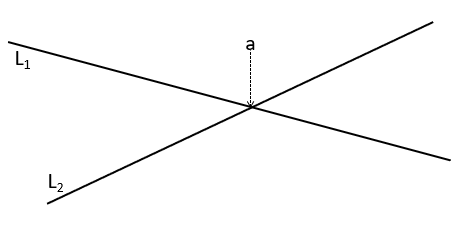
\includegraphics[width=1.0\textwidth]{Images/Prob1a.png}
    \caption{$n=2$}
  \end{minipage}
  \hfill
  \begin{minipage}[b]{0.3\textwidth}
    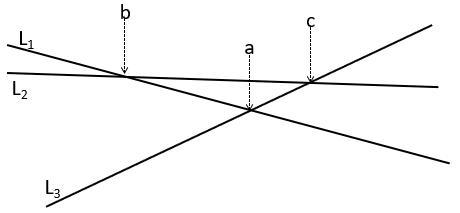
\includegraphics[width=1.0\textwidth]{Images/Prob1b.png}
    \caption{$n=3$, all lines visible}
  \end{minipage}
  \hfill
  \begin{minipage}[b]{0.3\textwidth}
    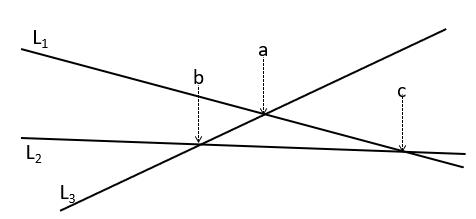
\includegraphics[width=1.0\textwidth]{Images/Prob1c.png}
    \caption{$n=3$, two lines visible}
  \end{minipage}
\end{figure}

When $n=2$, both $L_1$ and $L_2$ are visible.  
The line of smaller slope is visible for $x < x_a$, and the line of greater slope is visible for $x > x_a$, as shown in Figure \#1.
It can be observed that the following property must hold true for any $n$:  \newline
The lines of smallest and largest slope, $L_1$ and $L_n$, when ordered by increasing slope, must be visible in any graph.  
$L_1 > L_2 , \dots , L_n$ for sufficiently small $x$, just as $L_n > L_{n-1}, \dots , L_1$ for sufficiently large $x$.

From this observation, it follows that for $n=3$ there are two cases:  case \#1 - only $L_1$ and $L_3$ are visible, as in Figure \#2; case \#2 - all 3 lines are visible.
To determine whether $L_2$ is visible, simply compare its point of intersection with $L_1$, $b$, to the intersection of $L_1$ and $L_3$, $a$.  
If $x_b < x_a$, $L_2$ will be visible for $x_b < x < x_c$, where $c$ is the intersection of $L_2$ and $L_3$.  This case is shown in Figure \#3.

The algorithm's base case determines what situation exists given $n$, and then returns the set of visible lines $L$ and their corresponding points of intersection.

\noindent \textbf{Recursive Case and Termination:}

The recursive call of the algorithm splits the input list $L$ into two inputs of size $|L|/2$, and returns the set of visible lines and points of intersection.  Because $n$ decreases with each recursive call, such that $n' < n$.  Eventually, $n' \leq 3$, and will thus terminate the algorithm.

\noindent \textbf{Merging:}

Consider the lines in Figure \#4.  Let $R = \{L_1, L_2, L_3\}$ and $R' = \{L_4, L_5 \}$.
The recursive call for $R$ would return lines $L_1$ and $L_3$ as visible, while the recursive call for $R'$ would return both $L_4$ and $L_5$ as visible.
For all $x >$ the intersection of $L_3$ and $L_4$, $p_{int}$, the uppermost line will be in $R'$.  The final set of visible lines will thus be $L_1, L_3, L_4, L_5$.

\begin{figure}[h!]
	\label{Merge}
	\centering
	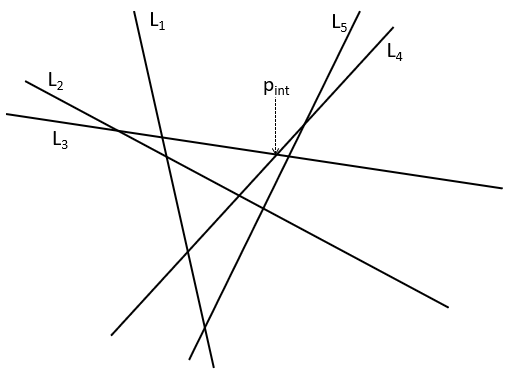
\includegraphics[scale=.5]{Images/RecursiveCase.png}
	\caption{Set of Lines 1-5, where $m_1 < m_2 < m_3 <m_4 < m_5$}
\end{figure}

This simply needs to be generalized, and the proof of merging will be satisfied. 
Define the set of points of intersection, $a$, such that $a_i$ is the intersection of lines $R_i$ and $R_{i+1}$, for any visible lines $R_i$ and $R_{i+1}$.
By sorting by increasing slopes, it guarantees that $a$ will be in order of increasing $x$ coordinate; and the set $b$, such that $b_i$ is the intersection of $R'_j$ and $R'_{j+1}$ for any visible lines $R'_j$ and $R'_{j+1}$.

Merge sets $a$ and $b$ into set $C$ by increasing $x$ coordinate.  
There exists some point, $c_k \in C$ where the uppermost line in $R'$ is above the uppermost line in $R$.  Assume the uppermost line in $R = R_i$ and the uppermost line in $R' = R'_j$.  Because $m_j > m_i$, the uppermost line for $x > c_k$ must satisfy $L_{uppermost} \in R'$.  
Let $p_{int}$ be the intersection of lines $R_i$ and $R'_j$.  All visible lines $l$ for $x < p_{int}$ must satisfy $l \in R$, and visible lines for $x > p_{int}$ must satisfy $l \in R'$.

The final set of visible lines $L_{final} = \{R_1, R_2, \dots , R_i \} \cup \{R'_j, R'_{j+1}, \dots , R'_n \}$.
The points of intersection, $C$, between the points will be $\{a_1, a_2, \dots a_{i-1} \} \cup \{p_{int}\} \cup \{b_j, b_{j+1}, \dots , b_{n-1} \}$.
Thus, because the algorithm determines the point $c_k$ where $R' > R$, and returns the corresponding list $L_{final}$; the result will be the proper merging of the visible lines from $R$ and $R'$.

\newpage

\section{Bipartite Matching Problem}

\subsection{Which algorithmic paradigm best describes this algorithm?}  
This algorithm is a greedy algorithm.

\subsection{Why did you choose the algorithmic paradigm selected above?}
It makes a local choice to add the first unmatched edge $e$ to the matching $M$, and terminates when there are no such edges remaining.

\subsection{Give an example of a bipartite graph $G$ for which this algorithm does not return the maximum matching.}
A bipartite graph $G$ which would not return the maximum matching is a path of length 3, where the middle edge is selected first. 
\begin{figure}[h!]
	\label{Bipartite}
	\centering
	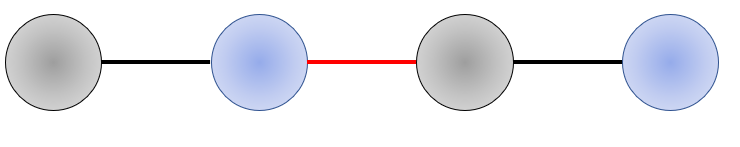
\includegraphics[scale=.5]{Images/Bipartite.png}
	\caption{Graph $G$ where the middle edge was selected first}
\end{figure}
The optimal matching would be to select the outer two edges, giving $|M'| = 2$.

\subsection{Let $M$ and $M'$ be matchings in a bipartite graph $G$.  Suppose that $|M'| > 2 \cdot |M|.$  Show that there is an edge $e' \in M'$ such that $M \cup {e'}$ is a matching in $G$.}

Any edge $e \in M$ or $e \in M'$ has two endpoints $p$ and $p'$, with $p \in X$ and $p' \in Y$.
Let $V'$ be the endpoints of $M'$, which gives $|V'| = 2 \cdot |M'|$.  
Let $V$ be the endpoints of $M$, which gives $|V| = 2 \cdot |M|$.

\begin{align*}
|M'| &> 2 \cdot |M|  \\
|M'| &> |V|
\end{align*}

\noindent Multiplying both sides by 2 and substituting in the relationship between $|M'|$ and $|V'|$, this gives the relationship $2 \cdot |M'| > 2 \cdot |V| \rightarrow |V'| > 2 \cdot |V|$.

Because any edge $e$ has two endpoints, 
$|V'| > 2 \cdot |V|$ implies $|V'| \geq 2 \cdot |V| + 2 $

The final observation needed is that half of the endpoints in any matching are in $X$, while the other half are in $Y$.  Thus,
$|V'_x| \geq |V| + 1$, and $|V'_y| \geq |V| + 1$.
Because $|V_x| = |V_y| = \frac{|V|}{2}$, it follows that there must be at least one edge $e$ that can be added to $M$ and still be a matching.  

A simplified way of stating the above claim is as follows:  because $|M'| > 2 \cdot |M|$, if every edge $e \in M$ has an endpoint in $M'$, there are still $>|M|$ possible edges remaining in $M'$.  Thus, the claim $|M'| > 2 \cdot |M|$ is false.

\subsection{Using the previous claim (and your supporting proof) to further prove that the algorithm is optimal or that the algorithm is $\rho$-optimal approximate (in this case be sure to derive the value of $\rho$ as part of your proof).}
As shown in part 3, the algorithm is not optimal because there exists a way to choose a non-optimal matching.
However, as shown in part 4, if $|M'| > 2 \cdot |M|$, there exists an edge $e$ such that $M \cup \{e\}$ produces a matching.  This edge would be found by the algorithm.  Thus, the below inequality must be true:
$$ |M'| \leq 2 \cdot |M| $$

\noindent This demonstrates that, although not optimal, the algorithm will be $\rho$-optimal for $\rho = \frac{1}{2}$, such that $|M| \geq \frac{M'}{2}$.

\newpage

\section{Number Partitioning Problem}

\subsection{Problem Statement:}  
Show that the \textit{Number Partitioning} is NP-complete using the \textit{Subset Sum} problem.

\subsection*{Show $Y \in$ NP}
Let $Y = Number \, Partitioning$.
Let $S$ be the set of all objects $1, 2, \dots , n$.  Assume we divided all $n$ objects such that $S_1 \subseteq S$, $S_2 \subseteq S$, and $S_1 \cup S_2 = S$.
Compute the value of each sum:
$$
V_1 = \sum_{i \in S_1} x_i  \hspace{1cm} V_2 = \sum_{i \in S_2} x_i
$$

\noindent If $V_1 = V_2$, the number partition exists and was found correctly.  This would require $O(n)$ operations because each item $i \in S$ belongs to either $S_1$ or $S_2$, and its value is added once.
The comparison $V_1 = V_2$ occurs in constant time.  
Thus, \textit{Number Partitioning} $\in NP$.

\subsection*{Choose an NP-Complete problem $X$:}
Let \textit{Subset Sum} be X.  \textit{Subset Sum} is NP-Complete by \textbf{8.23} \cite{algDesign}.

\subsection*{Prove that $X \leq_P Y$}
\textit{Subset Sum} determines, from a set of natural numbers $S$, whether there exists a subset of numbers $s'_i, \dots , s'_k$ such that $\sum_{i=1}^{k} s'_i = W$, for some target $W$.

Let $S$ be the set of objects $1, 2, \dots , n$.  
Find the sum, $X$, such that $X = \sum_{i=1}^n x_i$.  
Define the target, $W$ as $W = \frac{X}{2}$.  
It follows that $X - W = \frac{X}{2} = W$.

If this subset $S_1$ exists; $S$ can be partitioned into equal subsets $S_1$ and $S_2 = S - S_1$, such that:

$$
 \sum_{i \in S_1} x_i = \sum_{i \in S_2} x_i \, \mathrm{and} \, S_1 \cup S_2 = S
$$

\noindent Given two subsets, $S_1$ and $S_2$, whether or not their values are equal can be determined in $O(n)$ time.  
If the subset sum problem can be solved, its solution will also solve the number partitioning problem. \newline
\noindent Thus, \textit{Subset Sum} $\leq_P$ \textit{Number Partitioning}.  By \textbf{8.14}, \textit{Number Partitioning} is NP-Complete \cite{algDesign}.

\printbibliography

\end{document}
